\section{Zielsetzung}
Das Ziel des Franck-Hertz-Versuches ist es die Energiedifferenz zwischen dem Grundzustand und dem ersten angeregten Zustand zu bestimmen. Außerdem soll die Ionisierungsenergie und die Energieverteilung der Elektronen untersucht werden.

\section{Theoretische Grundlage}
\label{sec:Theorie}
\subsection{Aufbau des Franck-Hertz-Versuches}
Der Franck-Hertz-Versuch wird in einem evakuierten Glasbehälter durchgeführt, in dem sich ein Glühdraht, eine Beschleunigerelektrode und eine Auffängerelektrode befindet (siehe Abbildung \eqref{fig:Apparatur}). Außerdem befindet sich ein Tropfen Quecksilber, welcher bei Raumtemperatur nur zu einem Teil gasförmig ist und bei steigender Temperatur weiter verdampft, in dem Behälter. Der Glühdraht wird zur Erzeugung von freien Elektronen verwendet und zwischen dem Glühdraht und der Beschleunigerelektrode liegt die Beschleunigungsspannung $U_\text{B}$ an. Diese Spannung beschleunigt die freien Elektronen in die Richtung der Auffängerelektrode. Die Bremsspannung $U_\text{A}$ liegt zwischen der Auffängerelektrode und der Beschleunigerelektrode an. Die Brems- und die Beschleunigungsspannung können sepparat voneinander durch jeweils eine Gleichspannungsquelle geregelt werden. Außerdem wird die Heizspannung auf einen konstanten Wert eingestellt.

\begin{figure}[H]
  \centering
  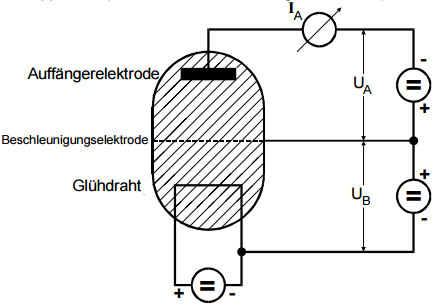
\includegraphics[height=7cm]{picture/Franck-Hertz-Apparatur}
  \caption{Schematischer Aufbau des Franck-Hertz-Versuches. \cite[2]{sample}}
  \label{fig:Apparatur}
\end{figure}

\subsection{Theorie}
Die beschleunigten Elektronen führen elastische und unelastische Stöße mit den Hg-Atomen aus. Die unelastischen Stöße treten immer dann auf, wenn das beschleunigte Elektron eine bestimmte Energie überschreitet und mit einem Hg-Atom zusammen stößt. Dadurch wird das Hg-Atom von seinem Grundzustand in seinen ersten angeregten Zustand angehoben und die Energiedifferenz der beiden Zustände lässt sich über
\begin{equation}
	\frac{m_0\, v_\text{vor}^2}{2} - \frac{m_0\, v_\text{nach}^2}{2} = E_1 - E_0
\end{equation}
berechnen, mit der Ruhemasse eines Elektrons $m_0$ und den Geschwindigkeiten $v_\text{vor}$ und $v_\text{nach}$. Die Energie der beschleunigten Elektronen vor dem Kollidieren beträgt
\begin{equation}
	\frac{m_0\, v_\text{vor}^2}{2} = e_0\, U_\text{B} \, ,
\end{equation}
wobei $e_0$ der Elementarladung und $U_\text{B}$ der Beschleunigungsspannung entspricht. Dies gilt allerdings nur für Elektronen, welche vorher keine kinetische Energie hatten. \\
Nach der Beschleunigerelektrode kommt eine Auffängerelektrode, zwischen diesen beiden liegt die Bremsspannung $U_\text{A}$ an. Dadurch kommen nur Elektronen mit einer kinetischen Energie in Feldrichtung zu der Auffängerelektrode, die die Ungleichung erfüllen:
\begin{equation}
	\frac{m_0\, v_\text{z}^2}{2} \ge e_0\, U_\text{A} \ .
\end{equation}
Der Rest der Elektronen kehrt zur Beschleunigungselektrode zurück. \\
Die Elektronen kollidieren mit den Hg-Atome auf zwei verschiedene Arten: elastisch und unelastisch. Der Energieverlust bei den elastischen Stößen, die nur auftreten, wenn das Elektron zu wenig Energie besitzt, kann vernachlässigt werden, da das Massenverhältnis $\frac{m_0}{M}$ zwischen dem Elektron und dem Hg-Atom sehr klein ist. Bei den unelastischen Stößen hingegen ist die Energie der Elektronen $E$ größer oder gleich der Energiedifferenz $E_1 - E_0$. Bei diesen Stößen gibt das Elektron diese Energiediffernz an das Hg-Atom, ab wodurch es in den ersten angeregten Zustand aufsteigt. Die überschüssige Energie bleibt bei dem Elektron. Nach $10^{-8}$\,s fällt das Hg-Atom wieder in den Grundzustand, wodurch ein Lichquant emittiert wird, welches die Energie
\begin{equation}
	h\, \nu = E_1 - E_0
	\label{eqn:EE}
\end{equation}
besitzt. Dabei ist $h$ das Planckschen Wirkungsquantum und $\nu$ die Frequenz der emittierten Strahlung. \\
In Abbildung \eqref{fig:Kurvenverlauf} ist der ideelle Verlauf des Strom $I_\text{A}$ in Abhängigkeit von der Beschleunigungsspannung $U_\text{B}$ zu sehen.

\begin{figure}[H]
	\centering
	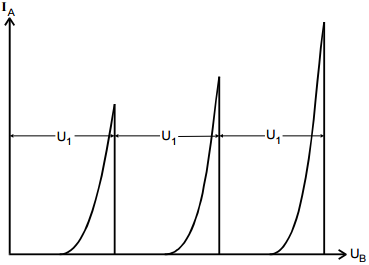
\includegraphics[height=6cm]{picture/Kurvenverlauf}
	\caption{Ideeller Kurvenverlauf von $U_\text{B}$ gegen $I_\text{A}$. \cite[4]{sample}}
	\label{fig:Kurvenverlauf}
\end{figure}

Die Beschleunigerspannung wird nun gleichmäßig nach oben gedreht und sobald diese größer als die Bremsspannung ist wird an der Auffängerelektrode ein ansteigender Strom registriert. Dieser Strom fällt allerdings abrupt ab sobald die Elektronen die Energiedifferenz $E_1 - E_0$ erreicht haben. Dies kann weitere Male passieren, wenn die Beschleunigerspannung groß genug ist. Die Distanz $U_1$ zwischen den Maxima der Kurve enspricht dem ersten Anregungspotential:
\begin{equation}
	U_1 = \frac{E_1 - E_0}{e_0}
\end{equation}
Der Kurvenverlauf aus Abbildung \eqref{fig:Kurvenverlauf} ist allerdings idealisiert und wird in der Praxis noch durch das Kontaktpotential, das Fermi-Dirac-Spektrum der Elektronen und den Dampfdruck beeinflusst. \\
\textbf{Das Kontaktpotential} kommt durch die unterschiedlichen Austrittsarbeiten des Glühdrahtes und der Beschleunigerelektrode zustande.

\begin{figure}[H]
	\centering
	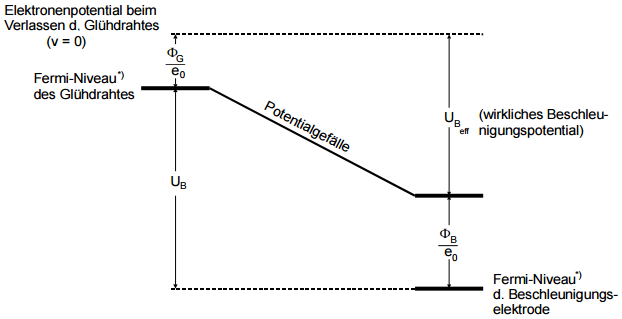
\includegraphics[height=7cm]{picture/Kontakt}
	\caption{Potentialverhältnisse zwischen Glühdraht und Beschleunigerelektrode. \cite[5]{sample}}
	\label{fig:Kontakt}
\end{figure}

Aus Abbildung \eqref{fig:Kontakt} kann die effektive Beschleunigungsspannung $U_\text{B, eff}$ abgeleitet werden
\begin{equation*}
	U_\text{B, eff} = U_\text{B} - K \ .
\end{equation*}
Der Summand $K$ entspricht dabei dem Kontaktpotential und hat den Wert
\begin{equation*}
	K = \frac{\Phi_\text{B} - \Phi_\text{G}}{e_0} \ ,
	\label{eqn:K}
\end{equation*}
wobei $\Phi_\text{B}$ der Austrittsarbeit der Beschleunigerelektrode und $\Phi_\text{G}$ der Austrittsarbeit des Glühdrahtes entspricht. Dadurch ist die Kurve um den Wert $K$ verschoben. \\
Die bisherige Annahme das alle Elektronen mit der selben Energie aus dem Glühdraht austreten stimmt nicht. Stattdessen treten die Elektronen entsprechend der Fermi-Dirac-Verteilung aus dem Glühdraht aus. Dadurch gibt es nicht nur eine Beschleunigungsspannung bei der die Elektronen die richtige Energie haben sondern einen Bereich indem das zutrifft. Aus diesem Grund gibt es nach dem Maximum keinen instantanen Abfall sondern eine stetig abfallende Kurve. \\
\textbf{Der Dampfdruck} beeinflusst die Häufigkeit der Zusammenstöße zwischen den Elektronen und den Hg-Atomen. Der Dampfdruck darf nicht zu niedrieg sein, da sonst kaum Elektronen mit dem Gas wechselwirken würden und ungebremst zur Auffängerelektrode fliegen könnten. Allerdings darf der Dampfdruck auch nicht zu hoch sein, da die Elektronen sonst zu oft mit dem Gas wechselwirken würden und garnicht mehr zur Auffängerelektrode gelangen würden. "Die mittlere freie Weglänge $\overline{w}$ der Atome muss klein gegen den Abstand $a$ zwischen Kathode und Beschleunigerelektrode sein" \cite[6]{sample}. Aus der Gastheorie folgt
\begin{equation*}
	\overline{w} = \frac{0.0029}{p_\text{Sät}} \ . \\
	\label{eqn:w}
	(\overline{w}\, [\text{cm}],\, p_\text{Sät} = \text{Sättigungsdampfdruck}\, [mbar])
\end{equation*}
Der Sättigungsdampfdruck lässt sich über
\begin{equation*}
	p_\text{Sät}(T) = 5.5 \cdot 10^7 \cdot \exp(\frac{-6876}{T}) \\
	\label{eqn:p}
	(T = Temperatur\, [K])
\end{equation*}
berechnen.

























\subsection{Fehlerrechnung}
Sämtliche Fehlerrechnungen werden mit Hilfe von Python 3.4.3 durchgeführt.
\subsubsection{Mittelwert}
Der Mittelwert einer Messreihe $x_\text{1}, ... ,x_\text{n}$ lässt sich durch die Formel
\begin{equation}
	\overline{x} = \frac{1}{N} \sum_{\text{k}=1}^\text{N} x_k
	\label{eqn:ave}
\end{equation}
berechnen. Die Standardabweichung des Mittelwertes beträgt
\begin{equation}
	\Delta \overline{x} = \sqrt{ \frac{1}{N(N-1)} \sum_{\text{k}=1}^\text{N} (x_\text{k} - \overline{x})^2}
	\label{eqn:std}
\end{equation}

\subsubsection{Gauß'sche Fehlerfortpflanzung}
Wenn $x_\text{1}, ..., x_\text{n}$ fehlerbehaftete Messgrößen im weiteren Verlauf benutzt werden, wird der neue Fehler $\Delta f$ mit Hilfe der Gaußschen Fehlerfortpflanzung angegeben.
\begin{equation}
	\Delta f = \sqrt{\sum_{\text{k}=1}^\text{N} \left( \frac{ \partial f}{\partial x_\text{k}} \right) ^2 \cdot (\Delta x_\text{k})^2}
	\label{eqn:var}
\end{equation}

\subsubsection{Lineare Regression}
Die Steigung und y-Achsenabschnitt einer Ausgleichsgeraden werden gegebenfalls mittels Linearen Regression berechnet.
\begin{equation}
	y = m \cdot x + b
	\label{eqn:reg}
\end{equation}
\begin{equation}
	m = \frac{ \overline{xy} - \overline{x} \overline{y} } {\overline{x^2} - \overline{x}^2}
	\label{eqn:reg_m}
\end{equation}
\begin{equation}
	b = \frac{ \overline{x^2}\overline{y} - \overline{x} \, \overline{xy}} { \overline{x^2} - \overline{x}^2}
	\label{eqn:reg_b}
\end{equation}
